\part*{Análisis y recomendaciones}

\section{Resultados}

% TODO: Explicar que hicimos 100 corridas
% TODO: Explicar los rotulos de los graficos (price_hours-0 y eso)

Previo al cálculo de los resultados, se calcuó el número $N$ de corridas necesarias para obtener valores dentro del intervalo de confianza deseado. En particular se buscaba 
un intervalo del 5\% con un nivel de significación del 99\%. El cálculo del número de corridas arrojó que 100 corridas serían suficientes para lograr estos niveles de confianza.\\

A continuación se presentan el cuadro de resultados, y los gráficos de las funciones objectivos, para estrategia de aceptación de recursos. Cabe destacar que las estrategias
están formadas por una combinación de 2 factores: la estrategia de aceptación en sí misma, y la cantidad de desarrolladores que se reservan para proyectos atractivos. Es por estos
que los rótulos tienen la siguiente forma: ``Nombre Estrategia - N devs'', como por ejemplo ``Precio HH - 2 devs'', que se refiere a la combinación de la estrategia 1 con 
2 desarrolladores reservados para proyectos atractivos.\\


\begin{table}[H]
\hspace*{-2cm}
 \begin{tabular}{|c|c|c|c|c|}
  \hline
  \multirow{2}{*}{\textbf{Estrategia}} & \textbf{Devs} & \textbf{Ingreso} & \textbf{Costo de Oportunidad} & \textbf{\% Recursos utilizados} \\
                                       & \textbf{Reservados}              &$[min, mean, max]$ & $[min, mean, max]$          & $[min, mean, max]$ \\
  \hline
  \hline
  \multirow{3}{*}{Precio HH}    & 0 &  $[124 : 128 : 131]$ & $[73 : 75 : 77]$ & $[19,5 : 20 : 20]$\\
  \multirow{3}{*}{}             & 2 & $[123 : 126 : 129]$ & $[74: 76 : 78]$ & $[19,5 : 20 : 20] $\\
                                & 4 & $[124 : 127 : 130]$ & $[75 : 76 : 78]$ & $[19,499 : 19,999 : 20]$\\
                                & 6 & $[124 : 127 : 131]$ & $[75 : 77 : 79]$ & $[19,493 : 19,993 : 20]$\\
  \hline
  \multirow{3}{*}{Facturación}  & 0 &  $[128 : 131 : 134$ & $[71 : 73 : 75]$ & $[19.5 : 20 : 20]$\\
  \multirow{3}{*}{}             & 2 & $[126 : 130 : 133$ & $[70 : 72 : 74]$ & $[19.5 : 20 : 20]$\\
                                & 4 & $[127 : 130 : 134$ & $[70 : 72 : 74]$ & $[19.498 : 19.998 : 20]$\\
                                & 6 & $[129 : 132 : 136$ & $[70 : 72 : 74]$ & $[19.5 : 20 : 20]$\\
  \hline
 \end{tabular}
 \caption{Resultados de la simulación}
\end{table}

\begin{figure}[H]

\begin{center}
    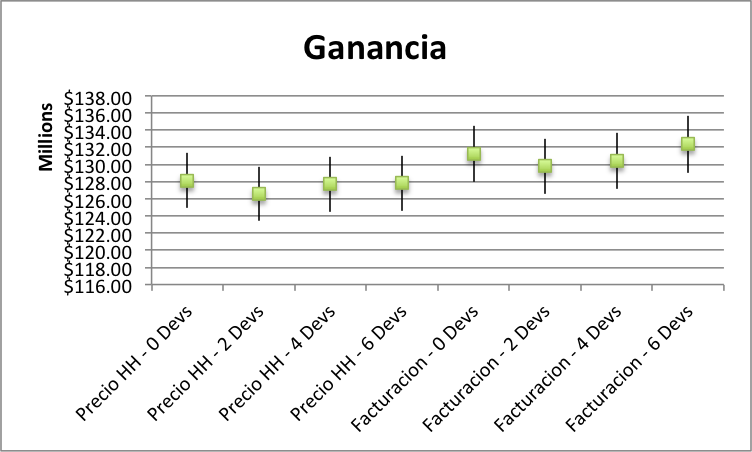
\includegraphics[width=0.75\textwidth,height=0.75\textheight,keepaspectratio]{./images/objective-earnings.png}
\end{center}

\label{fig:objective-earnings}
\caption{Ganancia con un intervalo del $5\%$ y $99\%$ de confianza}

\end{figure}

\begin{figure}[H]

\begin{center}
    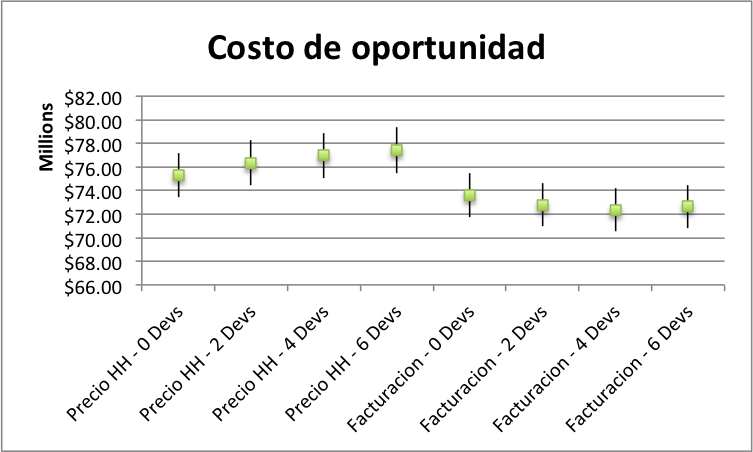
\includegraphics[width=0.75\textwidth,height=0.75\textheight,keepaspectratio]{./images/objective-cost.png}
\end{center}

\label{fig:objective-cost}
\caption{Costo de oportunidad con un intervalo del $5\%$ y $99\%$ de confianza}

\end{figure}

\begin{figure}[H]

\begin{center}
    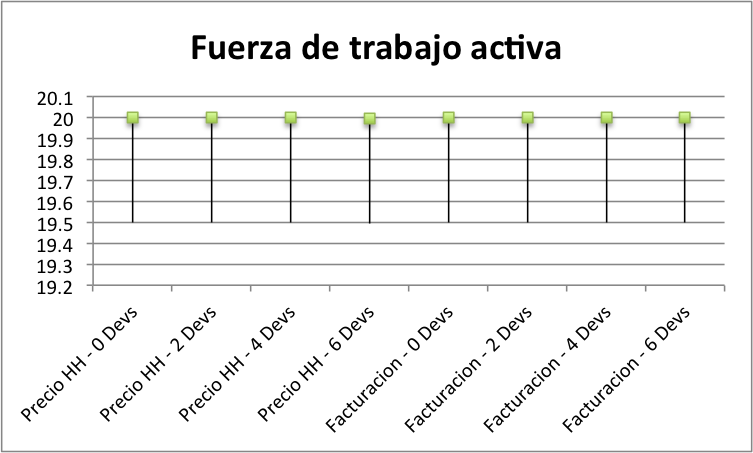
\includegraphics[width=0.75\textwidth,height=0.75\textheight,keepaspectratio]{./images/objetive-active-workforce.png}
\end{center}

\label{fig:objective-active-workforce}
\caption{Fuerza de trabajo activa con un intervalo del $5\%$ y $99\%$ de confianza}

\end{figure}

\section{Conclusiones}

Un resultado que salta a la vista es que ambas estrategias logran un aprovechamiento óptimo o cuasi-óptimo de los recursos (ambas mantienen ocupados siempre
o casi siempre a los 20 desarrolladores), por lo que no se puede basar solamente en este criterio para tomar una decisión acerca de que estrategia resulta más conveniente.
Esto puede deberse también al diseño de la estrategia de asignación de recursos, la cual utiliza siempre a los desarrolladores que no tienen trabajo asignado para colaborar con 
los proyectos en desarrollo, pero dejándolos disponibles para aceptar nuevos proyectos.\\

Los resultados muestran que si se tiene en cuenta la ganancia, no hay diferencias significativas, aunque se podría 
aventurar que la estrategia 2, la que se base en la facturación, podría ser levemente mejor. Por otro lado, si se tienen en 
cuenta el costo de oportunidad, si se observa una clara diferencia en favor de la estrategia 2, que tiene consistentemente un menor costo de 
oportunidad que la estrategia 1.\\

\section{Recomendación}

En vista de los resultados y el análisis realizado, la recomendación sería que se utilice la estrategia 2, basadándose en la facturación de los proyectos para su aceptación.
Queda claro que esto se da en un marco muy simplificado, con variables que fueron excluidas y aspectos que fueron desestimados para facilitar el desarrollo y el análisis de los
datos.\\

\section{Próximos pasos}

Algo interesante para agregar al simulador sería la inclusión de más estrategias de decisión, algunas más triviales y algunas más complejas, para comparar 
con las actuales y ver si realmente son tan buenas como parecen. \\

Además, en algunos casos parecería que tener una mayor cantidad de desarrolladores reservados podría hacer que alguna estrategia fuera mejor, con lo cual sería interesante
extender los rangos de valores para dicha variable de control y encontrar los puntos de quiebre para cada estrategia.\\

Otra mejora podría ser la consideración de crisis o períodos caóticos, en los que la demanda de proyectos se reduce notablemente o 
incluso se anula. Esto reflejaría las condicones de un mercado como el argentino, que se caracteriza por su inestabilidad, y mostraría como las 
estrategias se comportan ante la falta de trabajo asegurado.\\



